\section{Implementation}

\begin{figure}
\begin{centering}
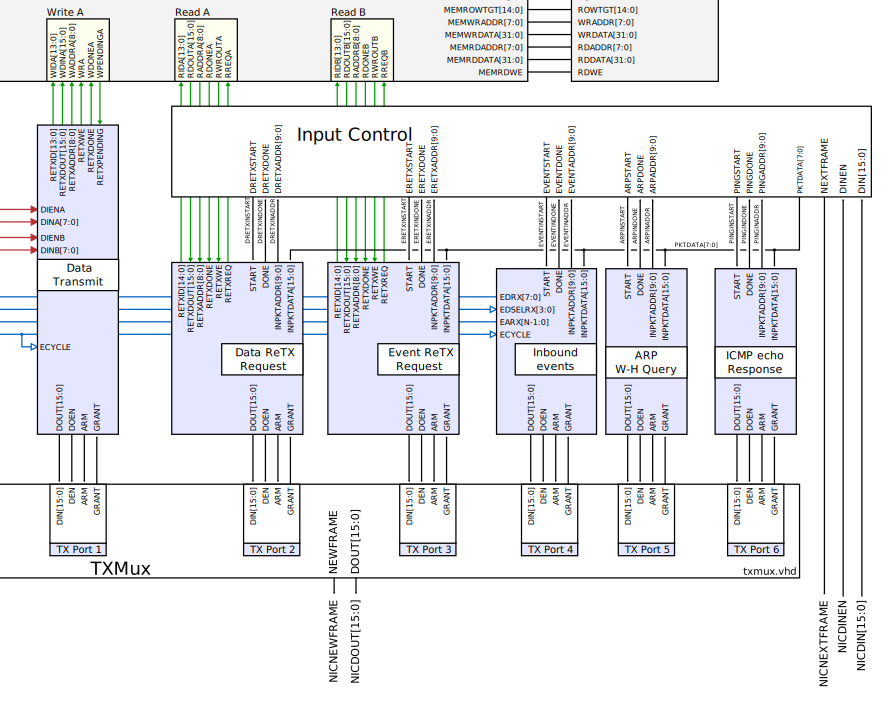
\includegraphics[scale=0.6]{overview.svg}
\end{centering}
\caption{A high-level view the Soma Network Stack architecture implementation.}
\label{overview}
\end{figure}

The Network Stack runs successfully at a 50 MHz clock with a
clock-doubled memory interface. 

The following global signals are used by nearly every module in the design: 

\begin{itemize}
\item \signal{MYIP[31:0]} 32-bit source IP address of the device. Defaults to 192.168.0.1. 
\item \signal{MYMAC[47:0]} 48-bit source MAC address of the device. Defaults to DE:AD:BE:EF:12:34. 
\item \signal{MYBCAST[31:0]} 32-bit broadcast IP address of the device; broadcast packets use this as their destination address. 
\end{itemize}

These signals can change at any time such that post-boot
reconfiguration of adresses can occur. Do not do this during
transmission of critical data, as it may result in invalid packet
transmission.

All data interfaces are 16-bits wide to match the IO requirements of
the soma Network Interface. All signals are active-high unless
otherwise indicated.


\subsection{Packet Processing Modules}
Most packet processing modules adhere to a common design: a single
multiplexed output buffer using a BlockRAM, which has the appropriate
constant values for the relevant frame set (for example, IP protocol
number and other header flags). The interface then writes the
per-packet unique data to this buffer, and transmits it out the
interface.


\subsection{Common Modules}
\subsubsection{IP Checksum}
\subsubsection{UDP Header Writer} 
